\section{Introduction}
\label{intro}

This document describes the use and development of the artifact search system developed as a Master's of Engineering thesis by Andrew Shafer at MIT.  This document assumes that the reader has a familiarity with MOOS and IvP and understands how to use those tools (see \cite{new03}, \cite{ben02a}, \cite{ben03}, and \cite{ben04b}).

First, a bit of terminology.  In this document, an "artifact" is an object of interest.  An artifact can be any detectable, identifiable object.  In a naval application this would commonly be some type of mine.  In naval terminology, "mine-hunting" (or mine-sweeping) usually refers to the process of detecting mines and deactivating or destroying them.  "Mine-searching," on the other hand, refers to simply mapping out the locations of detected mines for later deactivation/destruction.  Therefore, this project is more properly an artifact searching system, rather than a mine-hunting system.

A "search area" is the geographic region that the user desires to search (see Figure~\ref{searcharea}).  This area is broken up into uniform, discrete cells that together constitute the "search grid" (see Figure~\ref{searchgrid}).

\begin{figure}[ht]
\label{searcharea}
\begin{minipage}[c]{0.5\textwidth}
  \centering 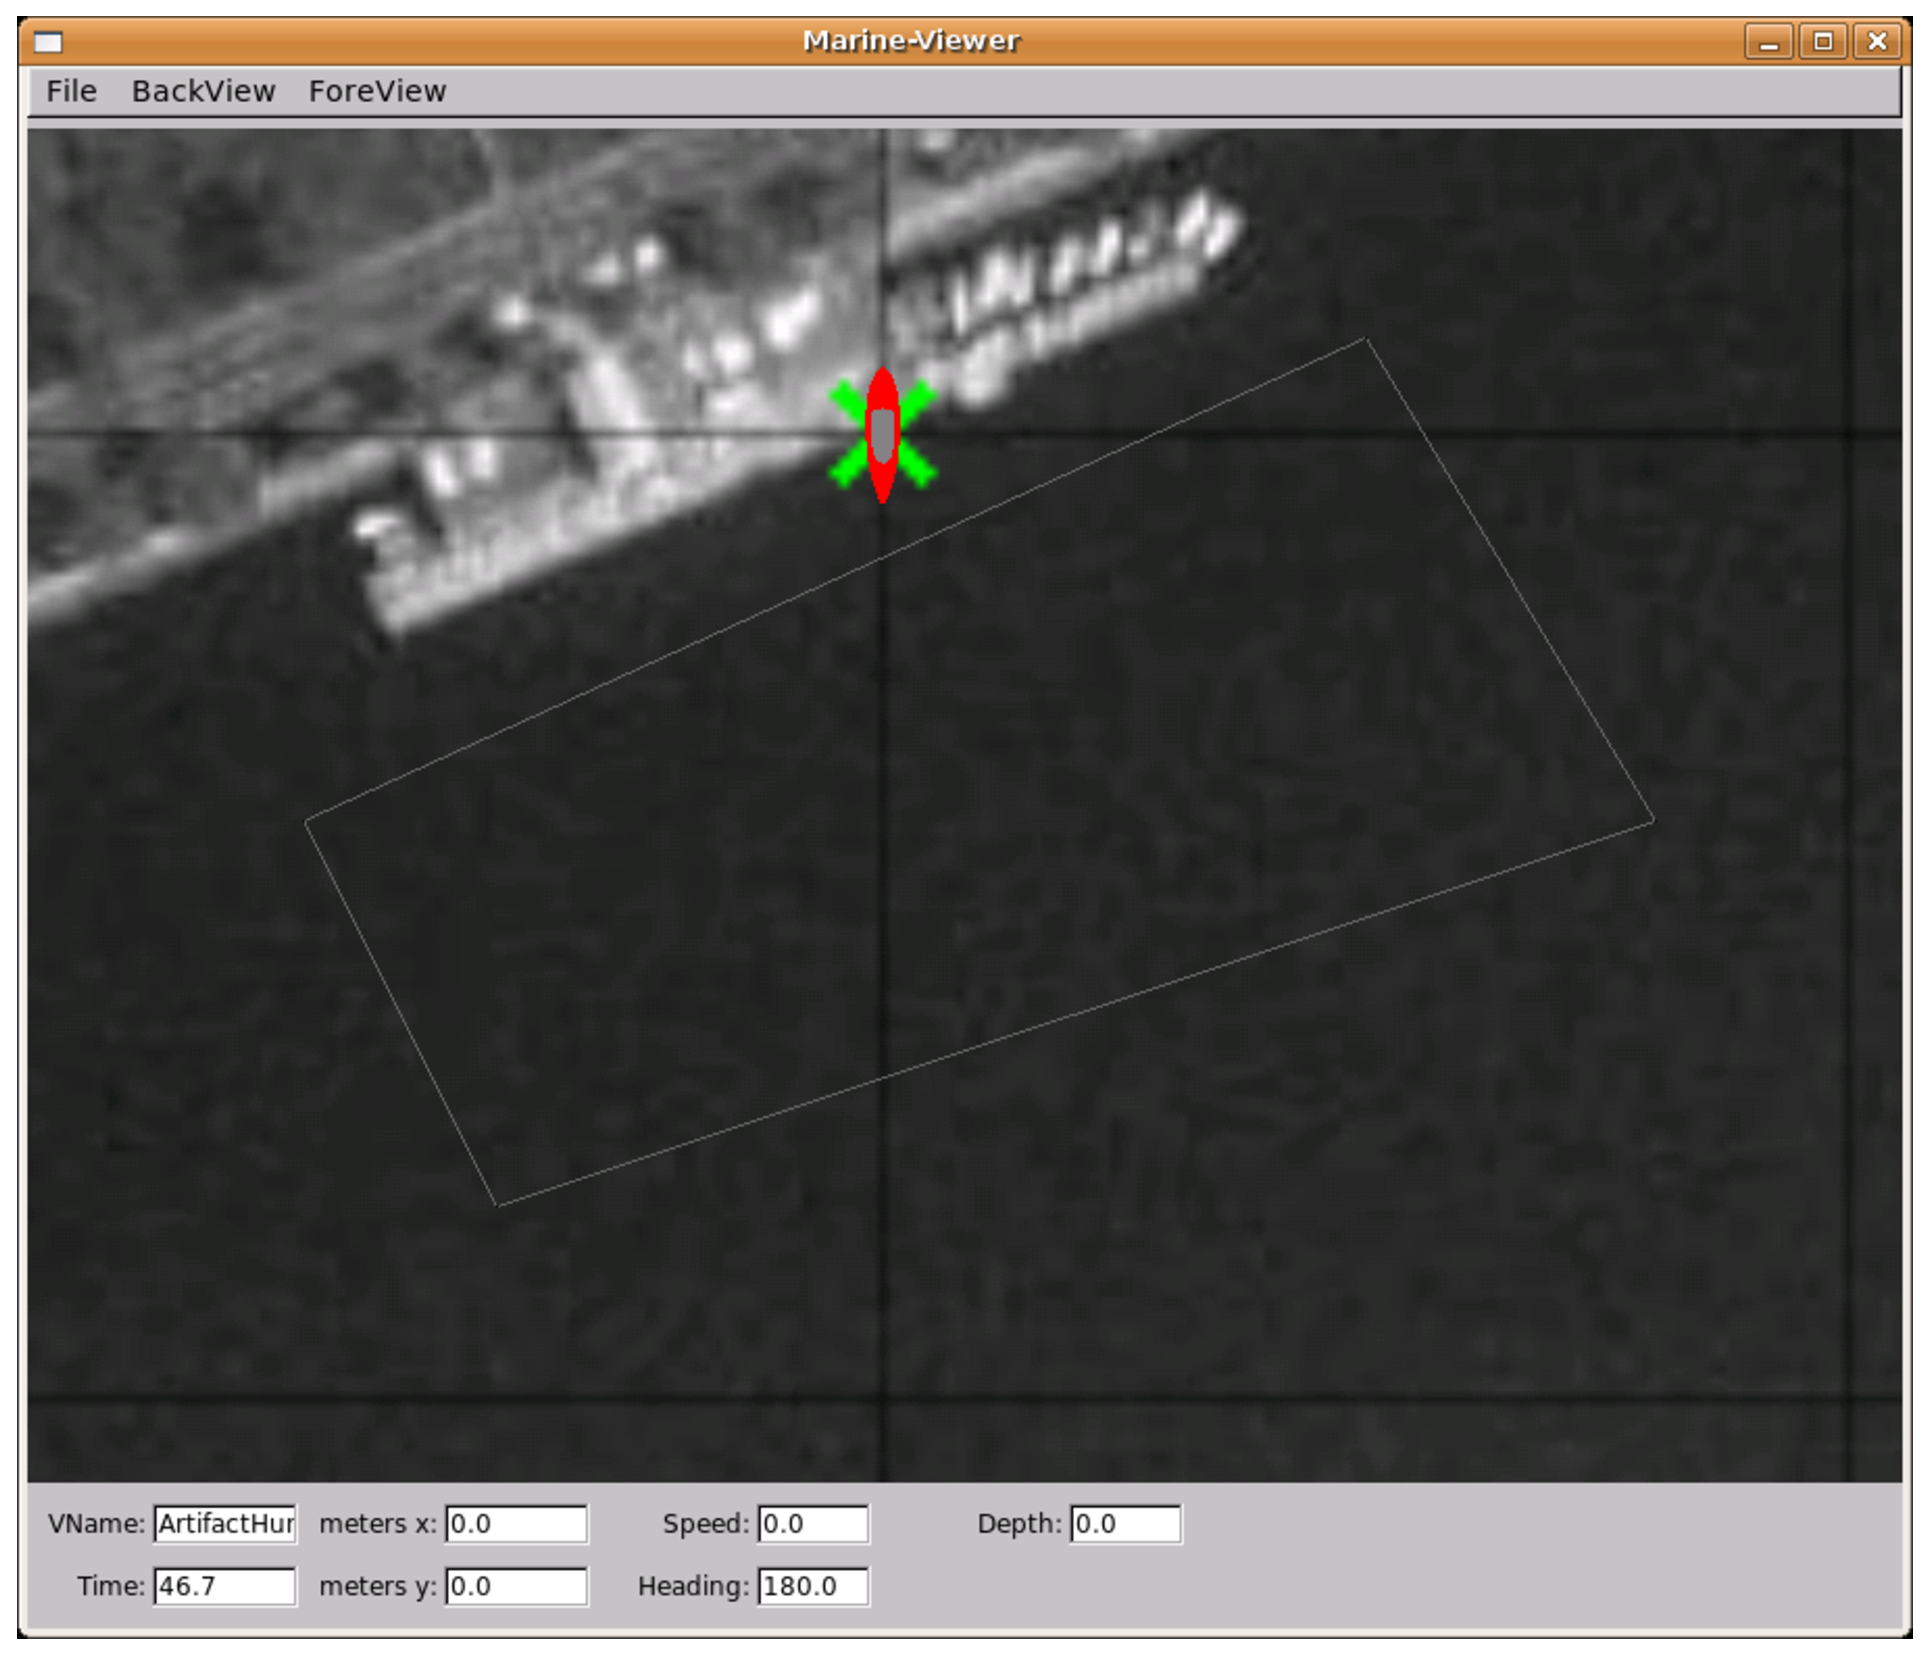
\includegraphics[width=2.5in]{figures/searcharea}
\end{minipage}
\caption{A geographic area (a convex polygon) defined as a search grid.}
\end{figure}

\begin{figure}[ht]
\label{searchgrid}
\begin{minipage}[c]{0.5\textwidth}
  \centering 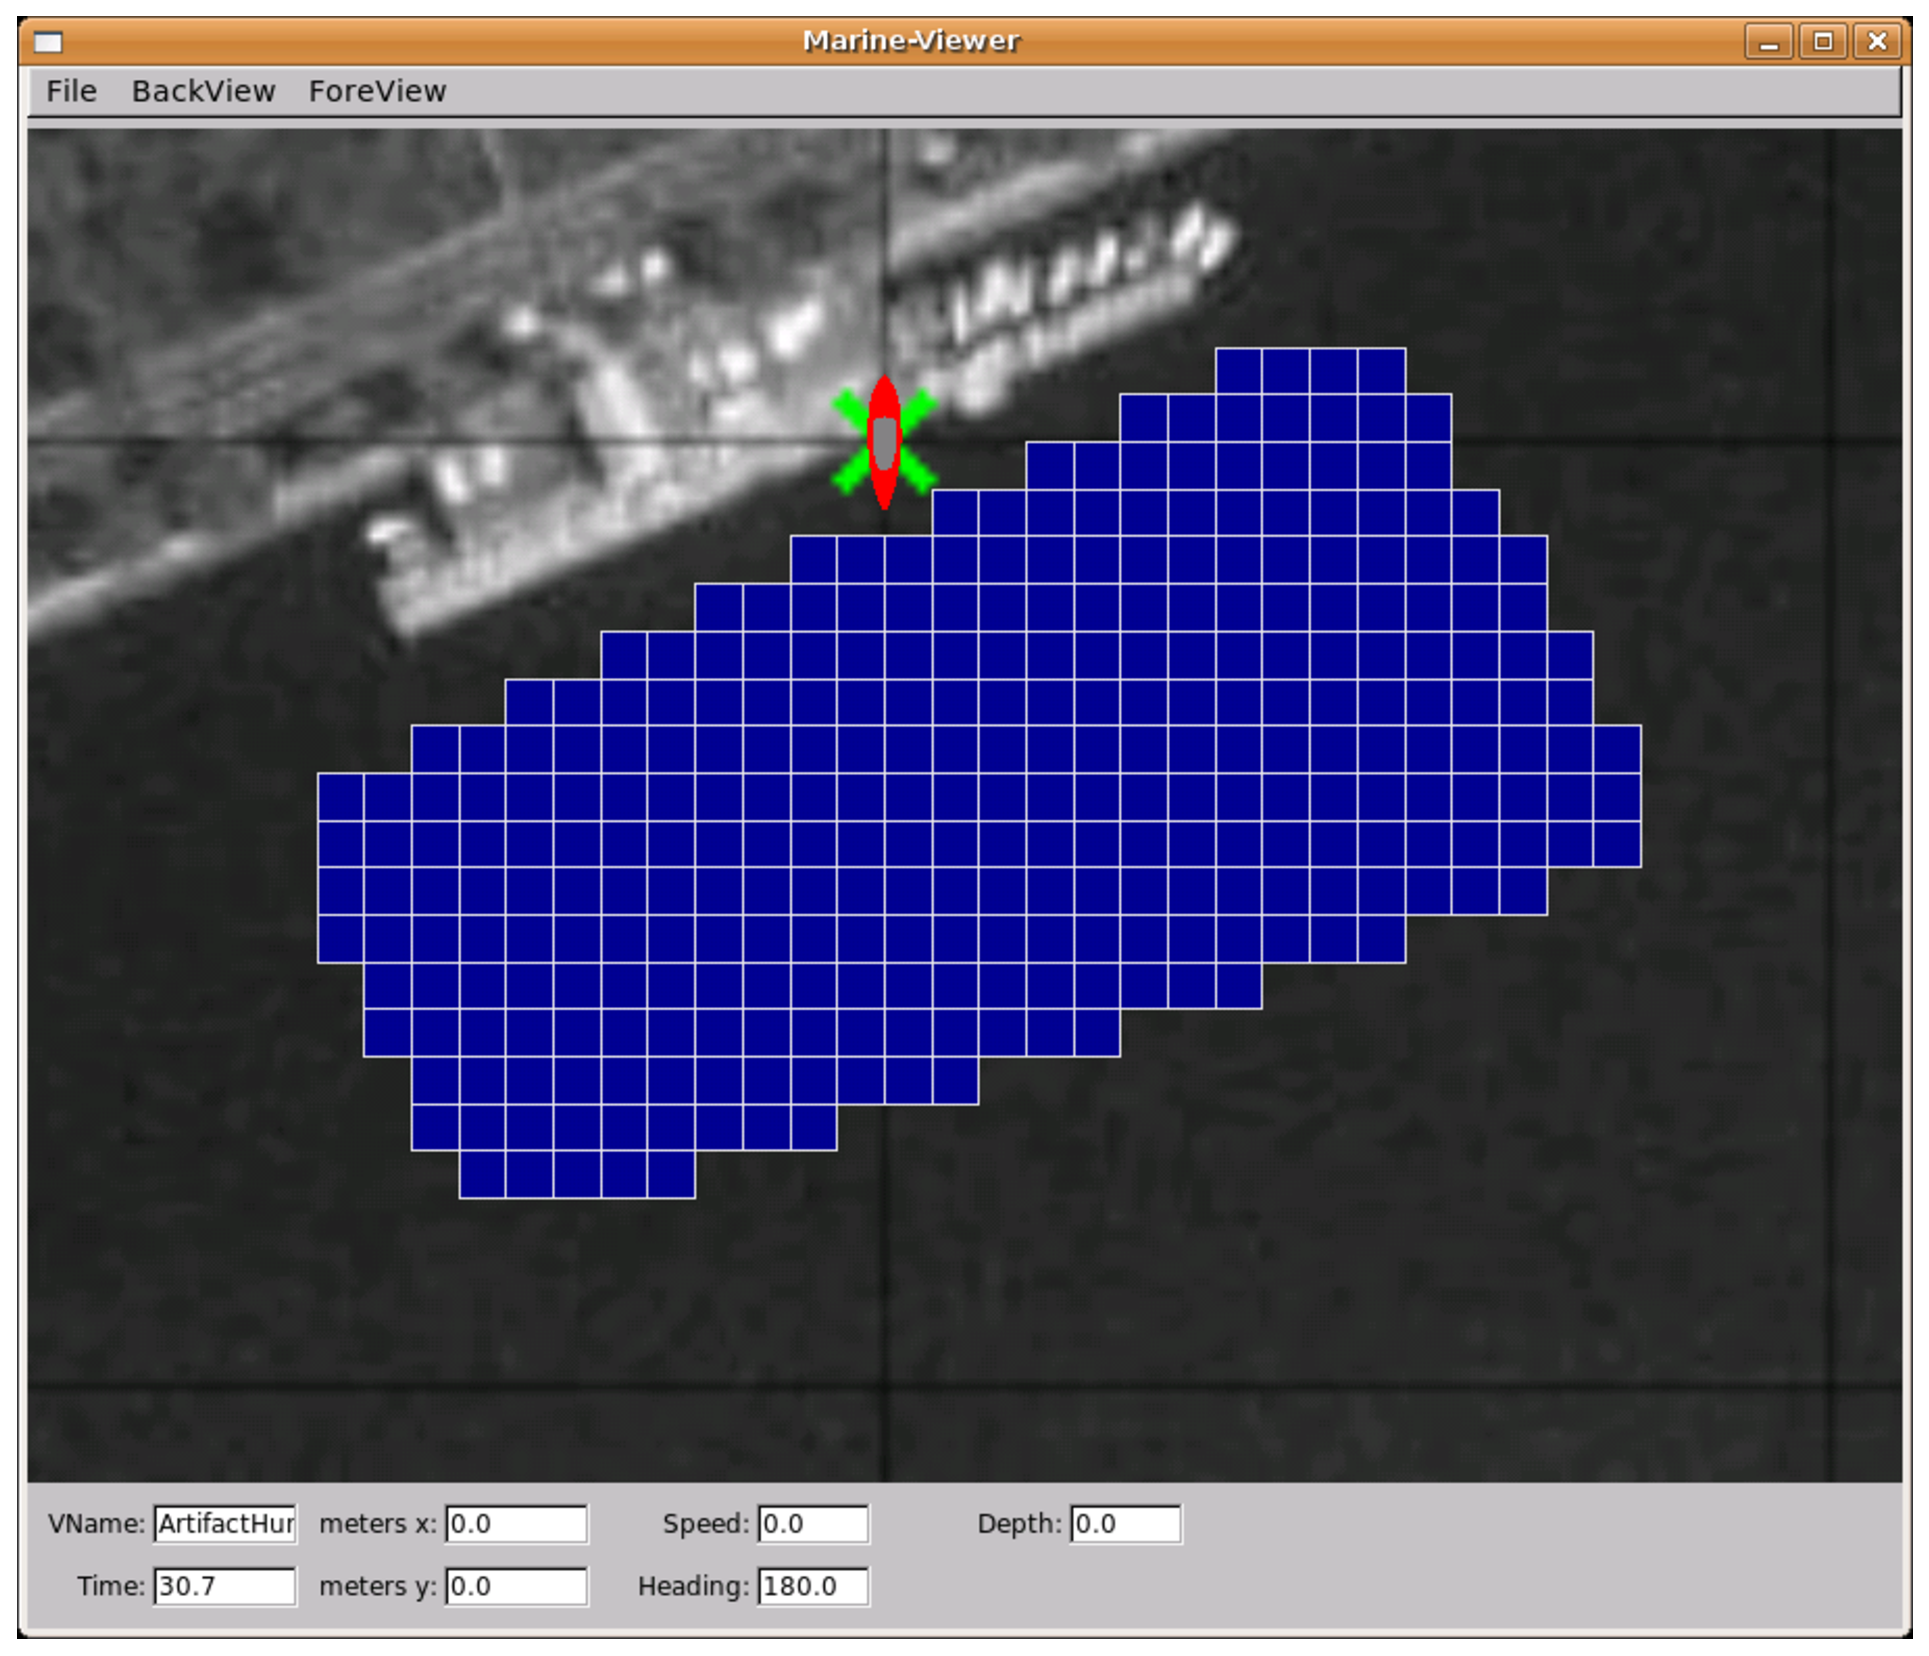
\includegraphics[width=2.5in]{figures/searchgrid}
\end{minipage}%
\caption{A search grid defined over a search area.} 
\end{figure}

There are two main MOOS processes and one IvPHelm behavior that implement the artifact search system.  pSensorSim simulates the output of an imaginary sensor in a simulated artifact field.  pArtifactMapper takes the output of pSensorSim, fuses it with output from other artifact search platforms in the area, and produces a likelihood map of artifacts in the search region.  The IvPHelm behavior, bhv\_SearchGrid, provides desired heading and speed information to the helm to optimize the user's utility function (e.g. mapping an entire field with 95\% confidence in the least amount of time).
% \begin{figure}[ht]
% \begin{minipage}[c]{0.5\textwidth}
%   \centering \includegraphics[width=2.5in]{figures/concept1.eps}
% \end{minipage}%
% \caption{The helm as a process in a MOOS community. \label{conceptone}} 
% \end{figure}
